
\documentclass[a4paper, 12pt]{report}

%%%%%%%%%%%%
% Packages %
%%%%%%%%%%%%

\usepackage[english]{babel}
\usepackage[noheader]{packages/sleek}
\usepackage{packages/sleek-title}
\usepackage{packages/sleek-theorems}
\usepackage{packages/sleek-listings}
\usepackage{longtable}

%%%%%%%%%%%%%%
% Title-page %
%%%%%%%%%%%%%%

\logo{figures/IFR_logo.png}
\institute{Canadian Light Source}
\faculty{FAR-IR Beamline}
%\department{Department of Anything but Psychology}
\title{The Interference-Fringe-Removal Project, V.0.1-beta}
\subtitle{FTIR spectroscopy interference fringe removal program.}
\author{\textit{Author}\\Jai \textsc{Willems}}
\supervisor{\textit{Supervisor}\\Brant \textsc{Billinghurst}}
\date{\today}

%%%%%%%%%%%%%%%%
% Bibliography %
%%%%%%%%%%%%%%%%

\addbibresource{./resources/bib/references.bib}

%%%%%%%%%%
% Others %
%%%%%%%%%%

\lstdefinestyle{latex}{
    language=TeX,
    style=default,
    %%%%%
    commentstyle=\ForestGreen,
    keywordstyle=\TrueBlue,
    stringstyle=\VeronicaPurple,
    emphstyle=\TrueBlue,
    %%%%%
    emph={LaTeX, usepackage, textit, textbf, textsc}
}

\FrameTBStyle{latex}

\def\tbs{\textbackslash}



%%%%%%%%%%%%
% Document %
%%%%%%%%%%%%

\begin{document}
    \maketitle
    \romantableofcontents
    
    
    % ----------------------------------------------------------------------
    % Introduction
    % ----------------------------------------------------------------------


    \chapter{Introduction to the IFR Program}
    
    \section{Introduction}
    The Interference-Fringe-Removal (IFR) program is a Windows-based application designed to enhance the removal of channel spectra by automating many areas of computation. Taking the form of a user interface, the IFR program allows a user to upload and inspect interferograms and spectral data to locate and select fringes. The program then returns the resulting spectra with the selected fringes removed.
    
    In the remaining chapters of this documentation, the program's operation and features will be discussed in addition to the program's methodology. For interested readers, the code will be broken down in the final pages to give a clear intuition of how the program works. But before all that, let us discuss the program's background and motivations.
    
    \section{Background}
    \subsection{The Michaelson Interferometer}

    The Michaelson Interferometer (figure \ref{fig:1}) is a key component to Fourier Transform Infrared (FTIR) spectroscopy to generate interferograms that can later be converted to spectra through a Fourier Transform.
    
    A light source enters the interferometer and contacts the beamsplitter at point C causing half to be directed to the mirror, M1, and the other half to the mirror M2. Upon reflection back to the beamsplitter, the beams recombine and are deflected to the detector at point E.
    
    \begin{figure}
        \centering
        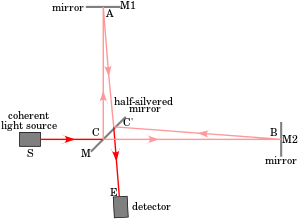
\includegraphics[width=0.5\textwidth]{figures/Michelson_interferometer.png}
        \caption{Michaelson Interferometer}
        \label{fig:1}
    \end{figure}
    
    The intensity of the light measured at the detector is affected by the pathlengths difference between the two mirrors, M1 and M2. When the interferometer takes measurements, one mirror will move while the other stays stationary, causing the pathlengths difference to evolve thereby allowing for a changing phase difference and thus varying degrees of constructive/destructive interference of the combining light waves. Consequently, the data gathered from the interferometer is a measure of the light's intensity against the mirror position and is known as an interferogram. By performing phase corrections and a Fourier transform, the resulting single beam spectrum can be calculated.
    
    \subsection{Interference Fringes \& The Effects on Data Collection}
    
    Due to the thickness of optics and windows present in the path of the light to the detector, light can bounce within the optics causing it to travel a different pathlengths difference thereby affecting the intensity of the light received at the detector. This can cause erroneous intensity readings known as interference fringes. Such fringes, if not properly removed, will appear as pseudo-sinusoids in the resulting spectrum when a Fourier Transform is performed. The pseudo-sinusoids can make data analysis more difficult when measuring intensities against an oscillating baseline or when fringe widths approach the width of absorption lines.
    
    \section{Motivation}
    The problem of an ideal fringe removal system is unsolved but there are methods to reduce their presence. The current method of the FAR-IR staff is a series of mathematical manipulations to find and subtract the fringe spectrum components from the final spectra. This methodology is time-intensive and can take upwards of an hour to remove one fringe. Large data sets can have up to 40 fringes. Consequently, the IFR program is designed to automate the calculations required to remove a fringe while maintaining user control over which fringes to include in the results.


    % ----------------------------------------------------------------------
    % Installation & Program Features
    % ----------------------------------------------------------------------
    
    
    \chapter{User Guide}

    \section{Download}

    The Windows executable file can be downloaded \href{https://github.com/JaiWillems/Interference-Fringe-Removal/releases/tag/v0.1-beta}{here} as \verb|IFR_v0.1-beta.exe| under the \textit{Assets} tab. Once downloaded, the program can be opened by double-clicking the application.
    
    Note that the above link will no longer be updated as of August 27th, 2021, contact the FAR-IR Beamline staff for the most up-to-date version.

    \section{Features}

    The Interference-Fringe-Removal program is a Windows-based user interface that contains various control categories.
    
    \begin{figure}[h]
        \centering
        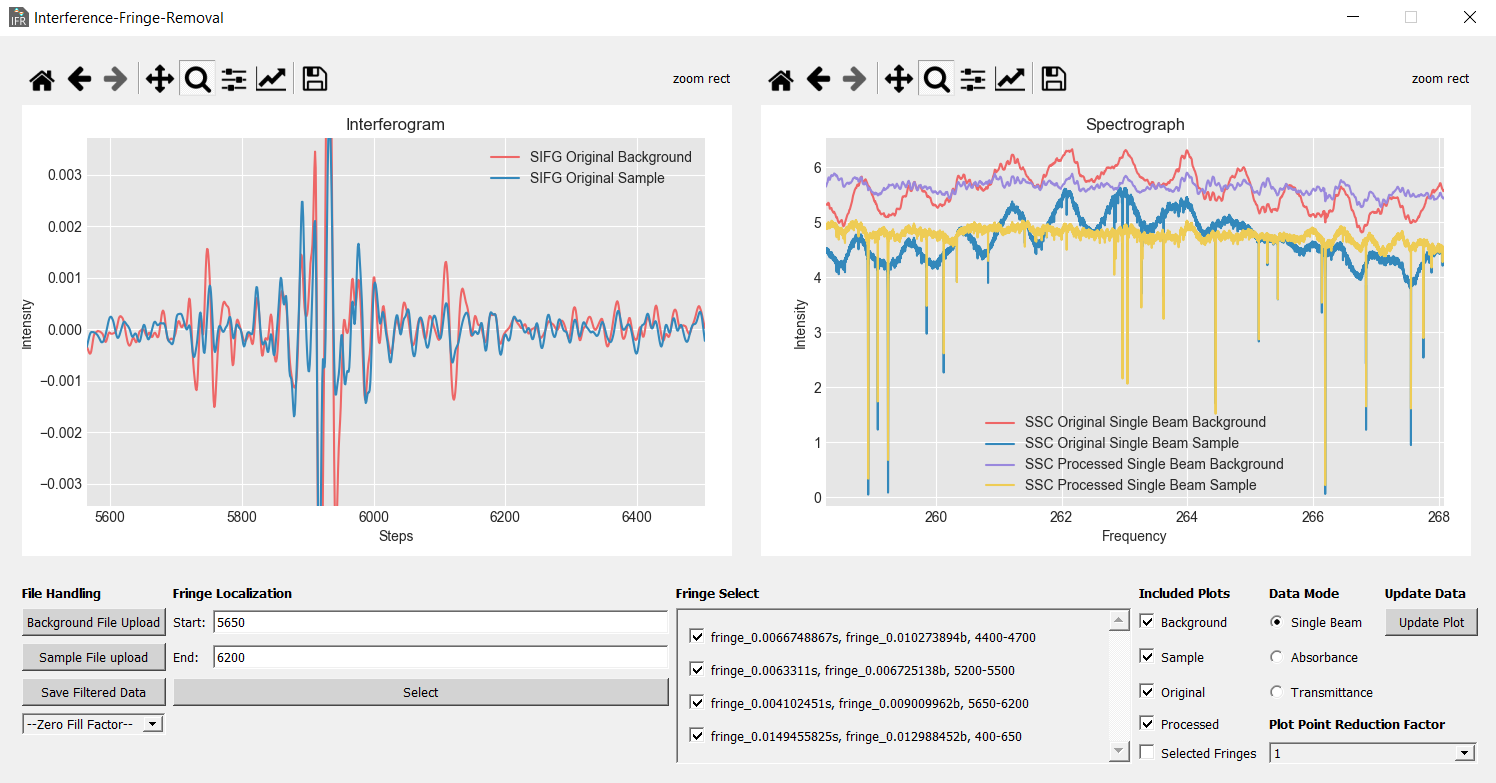
\includegraphics[width=\textwidth]{figures/ui_display.png}
        \caption{Interference-Fringe-Removal Program}
        \label{fig:2}
    \end{figure}
    
    \subsection{File Handling Controls}
    
    To use the IFR program, there is a need to be able to import OPUS file data and save processed spectra. Such functionality is gained from the file handling controls seen in figure \ref{fig:3}.
    
    \begin{figure}[h]
        \centering
        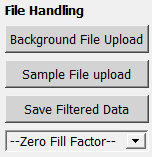
\includegraphics{figures/file_handling.png}
        \caption{File handling controls.}
        \label{fig:3}
    \end{figure}
    
    Sample and background data can be uploaded using the \textit{Sample File Upload} and \textit{Background File Upload} buttons, respectively. Most functionality including fringe localization, plotting transmittance and absorbance spectra, and saving processed data cannot be accomplished until both the sample and background data are uploaded.
    
    After processing a spectrum, the processed data can be zero-filled and saved as a \verb|.dpt| file. By pressing the \textit{Save Filtered Data} button, the program will zero-fill the spectrum data using the selected zero filling factor before saving all different spectra representations. For more information on the process, refer to section \ref{export_program_data}.

    \subsection{Fringe Localization \& Selection Controls}
    
    The primary functionality of the IFR program requires one to locate and remove selected fringes. A user can accomplish this using the fringe localization and selection controls as seen in figure \ref{fig:4}.
    
    \begin{figure}[h]
        \centering
        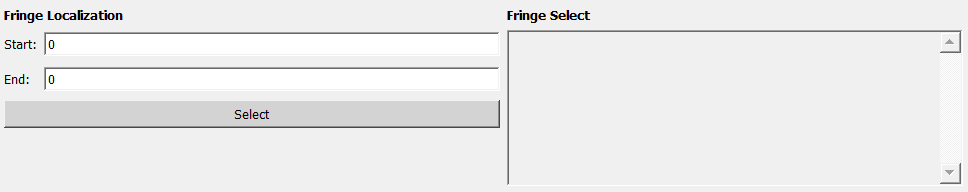
\includegraphics[width=\textwidth]{figures/fringe_controls.png}
        \caption{Fringe controls.}
        \label{fig:4}
    \end{figure}
    
    The first step in the fringe removal process is to locate a fringe. Navigating the interferogram plot, find the values on the x-axis that correspond to the start and end of a fringe. Input these fringe bounds into the \textit{Fringe Localization} line edits and press the \textit{Select} button to make the fringe appear in the \textit{Fringe Select} window. The fringe localization will run a series of calculations in the back before the fringe appears in the \textit{Fringe Select} window which can take several seconds. The steps to get the fringe spectrum component are detailed in section \ref{fringe_removal}.
    
    A localized fringe can then be selected for removal from a spectrum by selecting the checkbox adjacent to the desired fringe label in the \textit{Fringe Select} window. The selected fringes will then be removed from the spectra in the next update of the spectral plot.
    
    \subsection{Plotting Preference Controls}
    
    The \textit{Plotting Preference Controls} (seen in figure \ref{fig:5}) allows a user to configure the spectral plot and is broken into four sections.
    
    \begin{enumerate}
        \item The \textit{Included Plots} section allows users to detail which graphs to include on the spectral plot. Note that the greater number of plots displayed will result in a greater time to plot and greater latency in the user interface controls. Consequently, it is recommended to show only necessary plots.
        \item The \textit{Data Mode} section allows the user to choose the outputted display spectra as being either single beam, absorbance, or transmittance. The latter two require significantly more calculations and may take a moment to update.
        \item The \textit{Plot Point Reduction Factor} reduces the number of data points plotted by the selected factor. Thus, a plot point reduction factor of one will result in no point number reduction whereas a factor of two will halve the number of plotted points. The motivation behind this feature is to reduce program latency when highly detailed data is not necessary. It is recommended to use a large factor when zooming and panning the plots and then reduce the factor once the desired plot window is attained.
        \item The \textit{Update Data} section contains the \textit{Update Plot} button to re-plot spectral data with the most recent parameters from the previous three sections. Updating the plot requires a series of backend calculations to be completed. The more fringes that are to be removed, more data points that are being plotted, and the data mode will all factor into the time to update the plot.
    \end{enumerate}
    
    \begin{figure}[h]
        \centering
        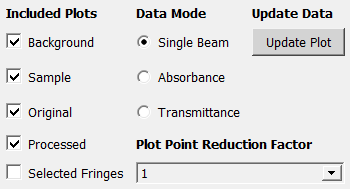
\includegraphics{figures/plot_preferences.png}
        \caption{Plot preference controls.}
        \label{fig:5}
    \end{figure}
    
    \subsection{Plot Controls}
    
    The plot controls seen in figure \ref{fig:6} are used to navigate the plot view. A brief description of each feature can be found \href{https://matplotlib.org/3.2.2/users/navigation_toolbar.html}{here}
    
    \begin{figure}[h]
        \centering
        
\includegraphics{figures/plot_controls.png}
        \caption{Plot controls.}
        \label{fig:6}
    \end{figure}
    
    
    % ----------------------------------------------------------------------
    % Program Methodology
    % ----------------------------------------------------------------------
    
    
    \chapter{Program Methodology}
    
    This chapter details the data handling methodology of the Interference-Fringe-Removal program.
    
    \section{OPUS File Preparation}
    
    The program uses prepossessed OPUS files as the data input. The program requires the data to be phase-corrected (both the interferogram and single beam spectra) and that the spectrum frequency range not be constrained. The steps to preprocess the data are as follows:
    
    \begin{enumerate}
        \item Import the data file of interest into OPUS.
        \item Select the interferogram data block and take the Fourier Transform. For the Fourier Transform options, select the Mertz phase correction and a frequency range set from 0 to 8000. It is also recommended to set the zero filling factor to one as higher factors will increase the latency of the IFR program. Zero filling can be accomplished with the IFR program when saving data.
        \item Once we have attained the phase-corrected single beam spectrum, we want to take the inverse Fourier Transform to get a phase-corrected interferogram. Take the Inverse Fourier Transform of the phase-corrected spectrum by selecting the single beam data block and applying an inverse Fourier Transform.
        \item Save the processed OPUS file data as an OPUS (\verb|.0|) file.
        \item Once steps 1 to 4 are completed for both the backgroud and sample data, import the files into the IFR program.
    \end{enumerate}
    
    \section{Modularized Operations}
    
    This section details smaller operations that will be used throughout the main processes outlined in section \ref{main_processes}.
    
    \subsection{Fast Fourier Transform}\label{fourier_transform}
    
    The Fourier Transform used in the program is a Hermitian Fast Fourier Transform which assumes the spectrum has Hermitian symmetry (i.e. a real spectrum). This assumption is based on the preprocessed input data being phase corrected. More detail on the Hermitian Fast Fourier Transform algorithm can be found \href{https://docs.scipy.org/doc/numpy-1.4.x/reference/routines.fft.html}{here} under the "Real and Hermitian Transforms" heading.
    
    \subsection{Zero Filling}\label{zero_fill}
    
    When a user saves processed data from the IFR program, they will have the option to zero-fill the data. Here, the zero filling factor will make the new data arrays a factor times longer. That is, if the initial data is $n$ long with a zero filling factor of $\alpha$, the zero-filled data will have a length of $\alpha n$. Zero filling is accomplished by appending $(\alpha - 1)n$ zeros to the dependent data array while the independent array is extended by appending an array of length $(\alpha - 1)n$ that ranges from $n+1$ to $\alpha n + 1$.
    
    \subsection{DataBlock Alignment}\label{DataBlock_alignment}
    
    The alignment operation in the IFR program takes two data sets and increases the number of data points in the shorter data array such that it has the same number of points as the larger data array. This allows for operations involving the two data sets. For example, to get the transmittance spectrum from the background and sample single beam spectra, we need to divide all data points in the sample spectrum by those in the background spectrum. Since background data is typically taken at a lower resolution, we need to increase the number of data points such that it matches the number of points in the sample spectrum before we ratio the two data sets.
    
    Alignment of the smaller spectrum data array to the larger spectrum data array is accomplished by taking the Inverse Fourier Transform of the spectrum, zero filling the resulting interferogram to the same number of points as the larger data set and then re-applying the Fast Fourier Transform to get the aligned spectrum. In this case, non-Hermitian Inverse Fourier Transform and Fast Fourier Transform algorithms are used as their effects on the data will cancel out and are faster to apply than their Hermitian counterparts.
    
    \section{Main Processes}\label{main_processes}
    
    This section details large processes employed within the IFR program.
    
    \subsection{Fringe Removal}\label{fringe_removal}
    
    The process of fringe removal from a spectrum requires the subtraction of the fringe's spectral component from the original spectrum. This process, as seen in figure \ref{fig:7}, follows the following workflow:
    
    \begin{itemize}
        \item Locate a fringe of interest in the spectrum's interferogram.
        \item Take all interferogram data up to and including the fringe (graph c) and apply the Fourier Transform to get the spectrum in graph e.
        \item Similarly, take all interferogram data up to and not including the fringe (graph d) and apply the Fourier Transform to get the spectrum in graph f.
        \item Subtract graph f from graph e to get the spectrum component due only to the fringe (graph g).
        \item Subtract the fringe spectrum component (graph g) from the original spectrum (graph a) to get the processed spectrum with the fringe removed (graph h).
        \item Iterate this process to remove all desired fringes.
    \end{itemize}
    
    \begin{figure}[h]
        \centering
        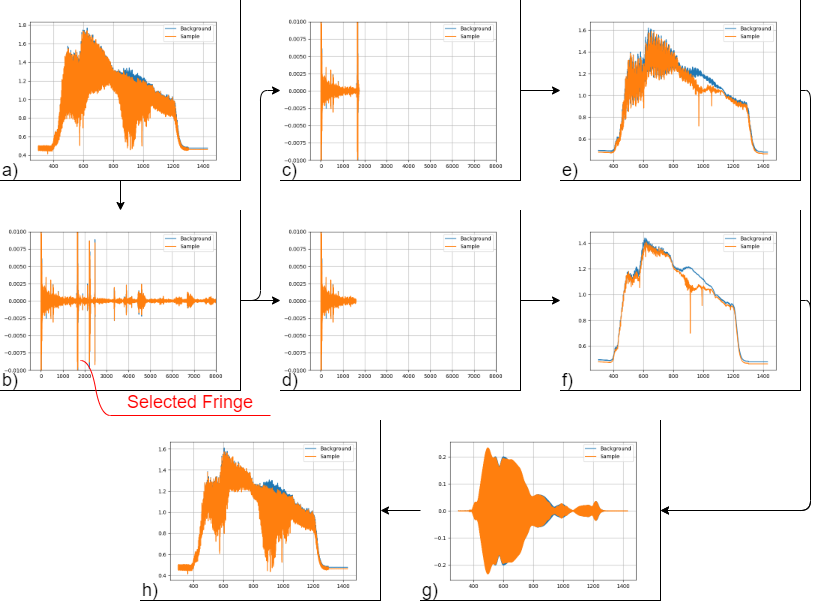
\includegraphics[width=\textwidth]{figures/poster_flow_chart_v3.png}
        \caption{Fringe removal flow chart.}
        \label{fig:7}
    \end{figure}
    
    \subsection{Calculating Transmittance \& Absorbance}\label{transmittance_and_absorbance}
    
    To calculate the transmittance and absorbance spectra, the IFR program first attains the sample and background single beam spectra with appropriate fringes removed. Using the methods in section \ref{DataBlock_alignment}, the program then aligns the background single beam spectrum such that it has the same number of points as the sample spectrum.
    
    The transmittance is then calculated by dividing the sample single beam intensities by the background single beam intensities. We then limit the range of the transmittance plot intensities from $-5$ to $5$. No useful transmittance data should lay outside this range. Without limiting the transmittance intensities, the absorbance values will grow large enough to cause overflow errors and issues importing the absorbance spectra into OPUS.
    
    The absorbance is calculated as $-\log_{10}(y_T)$ where $y_T$ is the transmittance intensity graph. By limiting the transmittance to between $-5$ and $5$, the absorbance intensities will be limited to a tolerable range. No useful absorbance data should be removed.
    
    \subsection{Exporting Program Data}\label{export_program_data}
    
    Exporting data from the program follows the following workflow:
    
    \begin{enumerate}
        \item Zero fill the background interferogram to the length of the sample interferogram and then by the zero fill factor.
        \item FFT the resulting interferogram to get the single beam spectrum.
        \item For each selected fringe, the fringe spectrum is calculated and subtracted from the background single beam as in section \ref{fringe_removal}.
        \item The background single beam with the background fringes removed is saved as a \verb|.dpt| file.
        \item Repeat steps 1 - 4 with the sample data.
        \item Calculate the transmittance and absorbance plots using the zero-filled background and sample data in accordance with the methods in section \ref{transmittance_and_absorbance}. Save the transmittance and absorbance data as \verb|.dpt| files.
        \item Export fringe locations as a \verb|.dpt| file.
    \end{enumerate}


    % ----------------------------------------------------------------------
    % MicroGUI Code
    % ----------------------------------------------------------------------
    
    
    \chapter{IFR Code}
    
    \section{File and Class Structure}
    
    The Interference-Fringe-Removal program is separated into seven source code files that combine to give the desired functionality.
    
    \begin{itemize}
        \item The \verb|main.py| script sets up the cache file system, initializes the \verb|UI| and \verb|Controller| classes, and removes the cache files after the program executes. This is the top level module used for the running the IFR program.
        \item The \verb|ui.py| file contains the \verb|UI| class which is responsible for creating the user interface by organizing the program's widgets.
        \item The \verb|controller.py| file contains the \verb|Controller| class which adds functionality to the user interface by connecting the interactive widgets defined in the \verb|UI| class to control sequences to update displays or process data.
        \item The \verb|definitions.py| file defines various path variables used in other files to interface with the cache file system.
        \item The \verb|dataobjects.py| file contains the \verb|OPUSData| class, \verb|DataBlock| class, and \verb|OPUSLoader| function to handle OPUS file data. The \verb|OPUSData| class is a simple data structure to hold all plot representations of an OPUS file. The \verb|DataBlock| class is a simple data structure to hold all information regarding a specific plot representation from an OPUS file. Lately, the \verb|OPUSLoader| is a convenience function which takes an OPUS file path and initializes the data structures to hold the file data.
        \item The \verb|operations.py| file contains the \verb|DataOperations| class which defines various data operations to apply to \verb|DataBlock| and Numpy array objects used throughout the IFR program.
        \item The \verb|compile_executable.py| file contains code that, when run, will create a program executable file.
    \end{itemize}
    
    \section{Imported Modules}
    
    This section details the various module imports used throughout the program. For each import, a brief description of its use and a reference to documentation will be given.
    
    For simplicity, only non-trivial and significant packages will be documented.
    
    \subsection{PyQt5}
    
    The PyQT5 package is a high-level API package used for the entire user interface. The documentation for the Python-based version is given \href{https://doc.bccnsoft.com/docs/PyQt5/}{here}.
    
    \subsection{Matplotlib}
    
    The Matplotlib package is designed to create data visualizations and animations in Python and is used for the plotting interfaces of the IFR program. Matplotlib documentation can be found \href{https://matplotlib.org/3.2.2/index.html}{here}.
    
    \subsection{Numpy}
    
    The Numpy package is a scientific computing Python library used in the IFR program for all data handling processes. Its documentation can be found \href{https://numpy.org/doc/stable/}{here}.
    
    \subsection{opusFC}
    
    The opusFC package allows the import of OPUS file data into Python. Its documentation can be found \href{https://stuart-cls.github.io/python-opusfc-dist/}{here}.
    
    \subsection{PyInstaller}
    
    The PyInstaller package bundles Python projects into program executables and is used by the IFR program to create the executable files. Its documentation can be found \href{https://pyinstaller.readthedocs.io/en/stable/usage.html}{here}.

\end{document}
